\section{Stable Matching}
The stable matching solves the problem of assigning one element $x \in X$ to another element $y \in Y$(for example: men to wimen, intern to hospitals, ecc...).

\begin{itemize}
	\item Unstable Pairs\\
	      A pair p(x,y) is defined as unstable if $\exists y^{*} \in Y \; such \;that \;p(x,y^{*}) > p(x,y) \; and \; vice-versa. $

	\item Stable Matching\\
	      A matching containing no unstable pairs.
\end{itemize}


\begin{figure}[h]
	\centering
	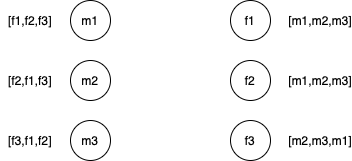
\includegraphics[width=0.4\textwidth ]{GS}
	\caption{An instance of the problem containing the M and W sets and $\forall m \in M, \; \forall w \in W$ a list of preferences for the elements in the opposite set, in increasing order.}
\end{figure}

\begin{figure}[h]
	\centering
	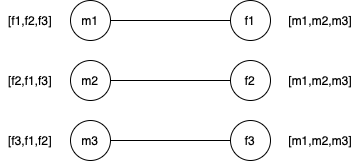
\includegraphics[width=0.4\textwidth ]{GS-Solved}
	\caption{A solution for the instance of the problem, containing only stable pairs.}
\end{figure}


\subsection{The Men-Wimen problem}
The problem about finding the stable matching between a set W and M. Each $w \in W$ rank every $m \in M$ from best to worst, and every $m \in M$ do the same.

\begin{algorithm}[H]
	\SetAlgoLined
	\small
	\KwIn{$M$ set of men, $W$ set of women}
	\KwOut{$S$ the set containing all the stable pairs between M and W}
	\BlankLine

	$S \leftarrow$ set containing all the pairs between M and W.

	\BlankLine
	\While{$\exists m \in M$ that is free and haven't proposed yet}{
	$w_{i} = m[0] \leftarrow$ first woman in m's list of preference to whom he is not yet proposed \;
	\If{$w_{i} \; is \; free$}{
	$S = S \cup p(m,w_{i}) \leftarrow$ create a pair between m and $w_{i}$\;
	}{
	}
	\BlankLine
	\If{$w_{i}$ prefers m to her current partner $m_{i}$}{
	$S = S - p(m_{i},w_{i})$\;
	$S = S \cup p(m,w_{i})$\;

	}{
	}
	\BlankLine

	}
	\BlankLine

	return $S$\;
	\caption{proposeAndReject(M, W) :}
\end{algorithm}

\begin{itemize}
	\item Observation 1\\
	      Every men propose to a women decreasing order of preference, for every women is the opposite.

	\item Observation 2\\
	      Once a women is matched she never become un-matched, she just change her partner, in increasing order of preference.

	\item Observation 3\\
	      Assuming $|M| = |W|$ then the algorithm has $\mathcal{O}(n^{2})$ complexity.

	\item Observation 4\\
	      The algorithm is very resistant to modifications: example new conditions on engagements.
\end{itemize}

\clearpage

